\documentclass[10pt,twocolumn,letterpaper]{article}

\usepackage{iccv_rebuttal}
\usepackage{times}
\usepackage{epsfig}
\usepackage{float}
\usepackage{graphicx}
\usepackage{amsmath}
\usepackage{amssymb}

% Include other packages here, before hyperref.

% If you comment hyperref and then uncomment it, you should delete
% egpaper.aux before re-running latex.  (Or just hit 'q' on the first latex
% run, let it finish, and you should be clear).
\usepackage[pagebackref=true,breaklinks=true,letterpaper=true,colorlinks,bookmarks=false]{hyperref}

%%%%%%%%% PAPER ID  - PLEASE UPDATE
\def\iccvPaperID{8604} % *** Enter the ICCV Paper ID here
\def\httilde{\mbox{\tt\raisebox{-.5ex}{\symbol{126}}}}

\begin{document}

%%%%%%%%% TITLE - PLEASE UPDATE
\title{STANLEY: Stochastic Gradient Anisotropic Langevin Dynamics for Learning Energy-Based Models}  % **** Enter the paper title here

\maketitle
\thispagestyle{empty}


%%%%%%%%% BODY TEXT - ENTER YOUR RESPONSE BELOW

We would like to thank the three reviewers for their feedback. 
Upon acceptance, we will include in the final version \emph{{\sf (a)} a clearer presentation of the algorithms} and \emph{{\sf (b)} additional experiments}. 
We address common concerns shared by the reviewers, noted R2, R3 and R4.

\noindent  \textbf{-- Notations (R2/R3):}
Upon acceptance, the revised paper will fix and include more comprehensive notations, particularly used throughout the theory section of our contribution.
The algorithm typos, in line 6, has been fixed (the stepsize does follow the EBM iteration index and not the MCMC iterations). We thank the reviewers for having pointed it out.

\noindent \textbf{-- Longer training procedures (R2/R3):}
Longer training procedure is a direction we will consider. 
Two options are possible: either increase the number of MCMC transitions per EBM iteration to make every chain convergent or increase the number of EBM iterations to reach better image quality.
For the former, our method aims at reducing the number of MCMC iterations which we exhibit by running non-convergent Markov chains. 
The latter option is doable and would increase the quality of the images generated with our method but also of all the other baselines.
Our purpose was to compare the algorithms at the same iteration threshold and compare their accuracies (FID and visually) regardless of reaching the optimal image quality after training.


\noindent \textbf{-- Additional numerical experiments (R2/R3/R4):}

We acknowledge the perfectibility of our contribution regarding numerical runs to convey the advantages brought by our STANLey update.
While we want to insist on the theoretical aspect of our method and on the fact that our runs on two different datasets are meant to illustrate the faster convergence of our method, we will add to the revised paper additional experiments including image translation and image completion/inpainting experiments.

\textit{More baselines:} Regarding our current numerical setup, which was to generate synthetic samples from the Flowers dataset and CIFAR-10, we add below additional baselines including the Langevin with a Metropolis-Hastings (MH) rejection step, the HMC sampler and a plain Gradient Descent (GD) without noise update of the samples.
Figure~\ref{fig:fidallmore} shows the FID curves for those new baselines vs. theSTANLey and plain Langevin sampler.
Additional synthetic samples after 100k EBM iterations for those new baselines can also be found  Figure~\ref{fig:cifarmore}.


\textit{Image inpainting:} 


\begin{figure}[t]
\begin{center}
\mbox{\hspace{-0.2in}
        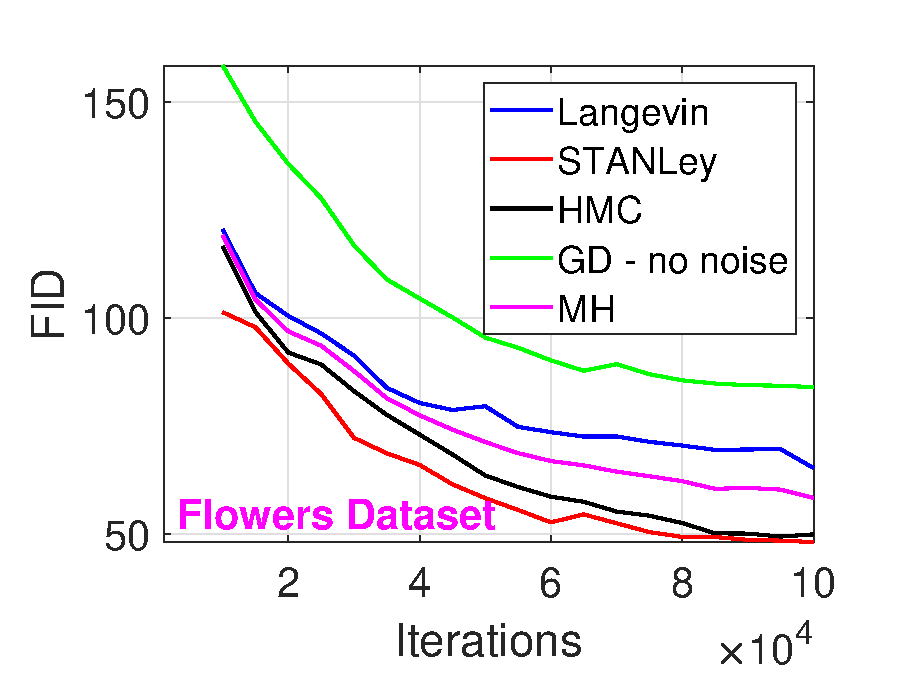
\includegraphics[width=1.9in]{figs/fid_flowersmore.eps} \hspace{-0.2in}
        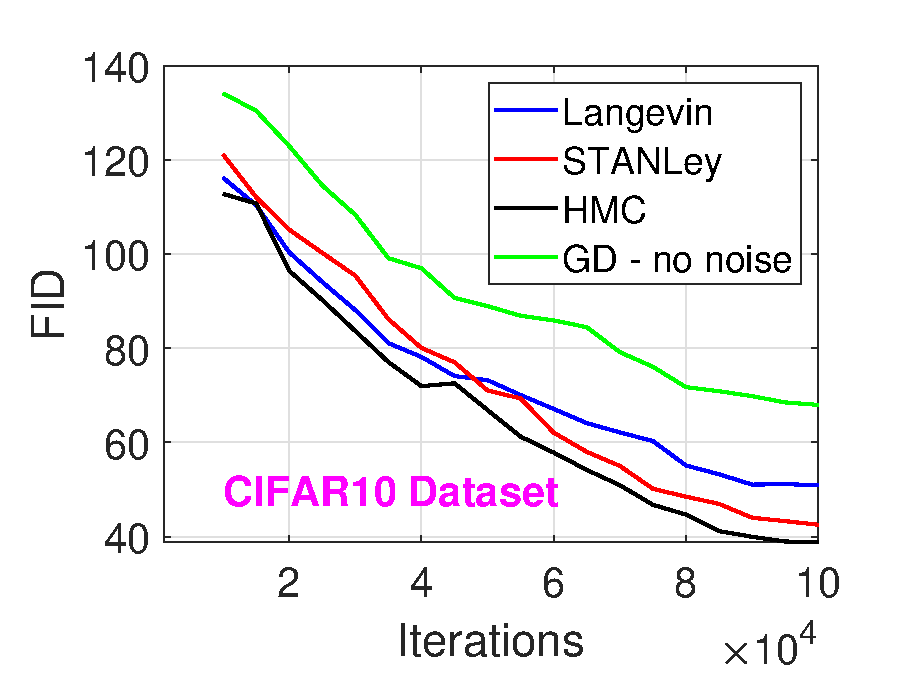
\includegraphics[width=1.9in]{figs/fid_cifarmore.eps}
        
}
\end{center}
	\caption{(FID values per method against 100k iterations elapsed). Left: Oxford Flowers dataset. Right: CIFAR-10 dataset.}
	\label{fig:fidallmore}
\end{figure}

\begin{figure}[t]
\begin{center}
    \mbox{
        \includegraphics[width=1.19in]{figs/cifaranila}
        \includegraphics[width=1.19in]{figs/mh_x_q_099900}
        }\vspace{0.05in}
            \mbox{
                \includegraphics[width=1.19in]{figs/hmc_x_q_099900}
                        \includegraphics[width=1.19in]{figs/gd_x_q_099900}
        }
\end{center}
\caption{(CIFAR Dataset). 1: STANLey 2: MH. 3: HMC 4: GD without noise. After 100k iterations.}
	\label{fig:cifarmore}
\end{figure}


\noindent \textbf{-- Originality of our contributions (R2/R3/R4):}
We would like to use a paragraph of our rebuttal to address all reviewers consideration of our paper.
We develop STANLey in order to more efficiently sample from the Gibbs potential. Hence, our goal is not to reach an optimal and high resolution generated image, but rather to decrease the number of kernel transitions need at each EBM iteration in order to obtain relatively good samples.
Drastically reducing this number would have a great impact on the energy consumption and speed of the whole training process.
Besides, we stress on the important theoretical contribution that is presented along our algorithm. 
To the best of our knowledge, EBM methods are presented mainly using empirical insights on their respective contribution.
In this paper, we wanted to show the benefit of using adaptive stepsize for learning a convent-based EBM where the energy landscape is highly nonconvex, not only via experiments but with a rigorous non-asymptotic convergence analysis.

This also echoes with R4's remark on "how the approach fits within the broader landscape of energy-based modeling approaches". 
Indeed, we specifically design STANLey update to take into account the curvature of the nonconvex energy landscape by embedding a dimension gradient informed stepsize.




% {\small
% \bibliographystyle{ieee}
% \bibliography{refrebuttal}
% }

\end{document}
